\begin{figure}
  \twoColsNoDivide{0.22}
  {
    \underline{$\Rep^R_K(\col)$}\\[2pt]
      $\salt \getsr \bits^\lambda$;
      $\pub \gets \langle 0^m, \salt, 0\rangle$\\
      for $x \in \col$ do \\
        $\tab \pub \gets \Up^R_K(\pub, \up_x)$\\
        $\tab$if $\pub = \bot$ then return $\bot$\\
      return $\pub$
  }
  {
    \underline{$\Qry^R_K(\langle M, \salt, c \rangle,\qry_x)$}\\[2pt]
      $X \gets \bmap_m(R_K(\salt \cat x))$\\
      return $M \AND X = X$
    \\[6pt]
    \underline{$\Up^R_K(\langle M, \salt, c \rangle,\up_x)$}\\[2pt]
      if $c \geq n$ then return $\bot$\\
      $M \gets M \vee \bmap_m(R_K(\salt \cat x))$\\
      return $\langle M, \salt, c+1 \rangle$
  }
  \caption{Keyed structure $\bloom[R,n,\lambda] = (\Rep^R,\Qry^R,\Up^R)$ is used
  to define Bloom filter variants used to rerpresent sets of at most~$n$
  elements. The parameters are a function $R: \keys\by\bits^* \to [m]^k$ and
  integers $n, \lambda \geq0$. A concrete scheme is given by a particular choice
  of parameters. The function~$\bmap_m$ is defined in Section~\ref{sec:prelims}.
  %
  }
  \label{fig:bf-def}
\end{figure}
In this section we consider two classes of Bloom filters, each employing a
different strategy to determine when the filter reaches full capacity. The first
class is specified in Figure~\ref{fig:bf-def}. This class of $n$-capped filters
captures the classical setting in which the filter is used to rperesent some
fixed number of elements $n\geq0$. Our construction $\bloom[R,n,\lambda] =
(\Rep^R,\Qry^R,\Up^R)$ has two additional parameters besides the cap: a
function~$R:\keys\by\bits^*\to[m]^k$ and the \emph{salt length}~$\lambda\geq0$.
%
Let $H:\bits^*\to[m]^k$ be a hash function and let $\ell, n, \lambda\geq0$ be
integers.
%
The standard Bloom filter is the structure $\BF[H,n] =
\bloom[\id^H,n,0]$, which we will term the \emph{basic} Bloom filter. It
has no key (the key sapce of $\id^H$ is $\{\emptystr\}$, see
Section~\ref{sec:prelims}) and does not use a salt.
%
The \emph{salted} Bloom filter $\SBF[H,n,\lambda] =
\bloom[\id^H,n,\lambda]$ is the same except that it allows a nonempty salt.
%
Finally, we consider a salted variant that uses a PRF instead of a hash
function. The \emph{keyed} Bloom filter $\KBF[F,n,\lambda]$ is the
structure $\bloom[F,n,\lambda]$, where $F:\keys\by\bits^*\to[m]^k$ is a
PRF.
%
Note that the basic and salted BFs have key spaces $\{\emptystr\}$ and the keyed
BF has key space~$\keys$.

In this section, we will show that the basic Bloom filter construction
$\BF[H,n]$ insecure in our setting. It allows the adversary to make an offline
attack that has a high probability of success while using a minimal number of
queries. In the immutable setting, where the adversary is constrained to never
use the $\UPO$ oracle, i.e. $q_U = 0$, it suffices to use the $\SBF$
construction in order to provide a security guarantee in either the
public-representation or private-representation settings. However, in the case
where we allow $q_U > 0$ so that the adversary can make updates, we will find
that $\SBF$ is only secure in the \erreps\ setting. To provide \errep\ security
when updates are needed, $\KBF$ must be used instead.

At the end of the section, we discuss the second class of filters that we call the
\emph{$\ell$-thresholded}. Instead of rejecting updates after a pre-determined
number of elements are added to the set, for these we decide the filter is full
once at leeast $\ell\geq0$ bits of the filter are set.
%
In the usual, non-adaptive setting, this strategy performs
similarly to the standard Bloom filter, but we find that a filter threshold
allows us to obtain better bounds.
%
We will demonstrate this for salted BFs in the \erreps\ setting.
%
\ignore{[...] and this construction has the additional advantage of not
requiring a separate counter to keep track of the number of elements in the
filter.}


\heading{Non-adaptive false-positive probability}
Let~$\rho:\bits^*[m]^k$ be a function, $\lambda\geq0$ be an integer, and
define $\bloom[\id^\rho,n,\lambda] = (\Rep^\rho, \Qry^\rho, \Up^\rho)$ as in
Figure~\ref{fig:bf-def}. (Note the mild abuse of notation by which we write
``$\rho$'' instead of ``$\id^\rho$''.)
%
Let $\setS\subseteq\bits^*$ be a set of length~$n$ and let
$x\in\bits^*\setminus\setS$. We define the non-adaptive, false positive
probability for Bloom filters as
\begin{equation}\label{eq:bf-fp}
  \begin{aligned}
    P_{k,m}(n) =
      \Pr\big[&\rho \getsr \Func(\bits^*,[m]^k);
              \pub \getsr \Rep^\rho(\setS): \\
              &\Qry^\rho(\pub, \qry_x) = 1 \given \pub \ne \bot
      \big] \,.
  \end{aligned}
\end{equation}
%
%(Note that, since the probability is conditioned on the event that
%$\pub\ne\bot$, this quantity is the same for both classes of filter.)
%
That is, $P_{k,m}(n)$ is the probability that some~$x$ is a false positive for
the representation of some~$\setS$ for which $|\setX|=n$ and $x\not\in\setS$,
when a random function is used for hashing.
%
Finding a tight, concrete upper bound for $P_{k,m}(n)$ has proven challenging,
but we do understand its asymptotic behavior. Kirsch and
Mitzenmacher~\cite{kirsch2006less} prove that, for certain choices of $k$ and
$m$ as functions of~$n$, it holds that
$
  P_{k,m}(n) = \lim_{n\goesto\infty} (1-e^{-kn/m})^k \,.
$
%
Moreover, they demonstrate via simulation that this is a very good approximation
of the false positive probability.
%
In lieu of a concrete upper bound, we will refer to $P_{k,m}(n)$ as defined in
Equation~(\ref{eq:bf-fp}) in the remainder.

\heading{Error function for set-membership queries}
%
Throughout this section we will use the error function~$\delta$ defined as
\begin{equation}
  \delta(x, y) =
  \begin{cases}
    0 & \text{if}\ x=y \\
    1 & \text{otherwise.}
  \end{cases}
\end{equation}
This simply indicates whether the query result matched the correct response.

\subsection{Insecurity of unsalted BFs}
The performance of basic Bloom filters is well-understood assuming the choice of
set~$\S$ being represented is independent of the choice of hash function. When
this assumption is violated, however, their performance can be substantially
degraded~\cite{gerbet2015power}.
%
Here we show that, even when we (optimistically) model the hash function as a
random oracle, basic BFs cannot achieve security in our setting.
%
The basic Bloom filter has no salt and no secret key.
Let $H:\bits^*\to[m]^k$ be a function, fix $n\geq0$, and let
$\Pi = \BF[H,n]=(\Rep^H,\Qry^H,\Up^H)$ as defined above.
%
With no per-representation randomness and no secret key to be concealed from the
adversary, there is no difference between \errep\ and \erreps\ security, as the
adversary can easily compute the representation of any set for itself. This
ability of the adversary to reconstruct the set without making queries allows
for various attacks that badly harm the accuracy of the filter.

\heading{Pollution attacks}
Gerbet \etal~\cite{gerbet2015power} provide the following example of an attack
setting and a potential attack against Bloom filters.
Suppose the adversary is interacting with a system representing a dataset
with~$\Pi$ and that it is able to choose some fraction of the input data.  For
example, consider a web crawler which performs a ``crawl'' of webpages
\cpnote{Maybe we should cite Google's white paper on Search?}, following
the links on each page it visits in order to index, archive, or otherwise
analyze websites. In order to keep track of the set of webpages which have
already been visited during a crawl, some crawlers use a Bloom filter which is
updated to include each new page the crawler visits.
Suppose the adversary controls at least one such webpage along the crawl's path
and wishes to deny the spider access to a different webpage, the `target
webpage'. The adversary can choose the links present on its own webpage, which
will cause the spider to visit the chosen webpages and set the corresponding
bits of its Bloom filter to~$1$. If those links are chosen in such a way that they
produce a false positive for the target webpage, the spider will then
erroneously believe it has already visited the target webpage. The target
webpage will therefore never be visited during the spider's crawl.

In cases where the adversary is able to control at least some of the filter inputs,
the authors describe an attack where the adversary chooses a set of
inputs that maximizes the number of 1s in the filter. This strategy is especially
effective when the structure of the hash function is known to the adversary. In
particular, as long as the choice of hash function and any associated parameters
are public, the adversary can compute the hash function on its own in order to
determine which choices will set the maximum number of bits to 1, or which
choices will set certain target bits to 1 in order to cause specific false
positives. They show that with $m = 3200$ and $k = 4$, the adversary can double
the false positive rate if they control 200 out of a total of $n = 600$
insertions, under the assumption that~$H$ is arbitrary but known to and
computable by the attacker.

Gerbet \etal suggest various ways to mitigate pollution attacks, such as choosing
the parameters $k$, $m$, and $n$ so that even if a pollution attack
occurs, the false positive rate is kept below some threshold of acceptability.
This strategy is  potentially viable, but may significantly increase the amount
of memory required to store the data structure.  The bounds we provide show how
the parameters of a filter can be tweaked to keep the error rate low not just in
the presence of this specific type of attack, but in the presence of any
adversary covered by our more general attack model; doing so, however, will
require altering the structure.

The authors also discuss the possibility of using a secretly-keyed
hash function. In the attack model they consider, where representations are kept
private indefinitely, this suffices to prevent the pollution attack they
describe. However, under the more general attack models where the representation
may eventually be recovered (in the private-representation setting via~$\REVO$)
or is public.  Simply using a PRF \emph{without per-representation randomness}
does not suffice for security in our setting.

\heading{Target-set coverage attacks}
%
Of course, exhibiting a high false positive rate is not the only way a Bloom
filter might fail to be correct. In particular, it would be undesirable if the
filter were consistently incorrect on a \emph{particular set of inputs}. Rather
than pollute the filter, the adversary's goal might be to craft a set of
legitimate looking inputs that cover some disjoint target set of inputs.
%
This type of attack is nicely captured by our adversarial model.
%
In a \emph{target-set coverage attack}, the adversary is given a small target set
$\setT\subseteq\bits^*$ and searches for a cover set $\setR\subseteq\bits^*$
such that $\Qry^H(\Rep^H(\setR),\qry_x)=1$ for each $x\in\setT$.
%
Once a suitable cover set is found, the adversary queries $\REPO(\setR)$. Then
for each $x\in\setT$, it asks $\QRYO(\qry_x)$, achieving a score of $r = |\setT|$.

This \erreps1 attack succeeds with probability~$1$ assuming a covering set can
be found.  If $|\setT| \leq |\setR|$, then such a set exists; but finding it may be
computationally infeasible, depending on the size of the cover set, the size of
the target set, and the parameters of the Bloom filter.
%
In Appendix~\ref{app:unsalted-attack} we demonstrate that target-set coverage
attacks are feasible for practical BF parameters. We do so by simulating the
attack when~$H$ is a random function (i.e., for each distinct input we choose
$k$ integers from $[m]$ at random) for typical choices of $k$, $m$, and~$n$.

\ignore{
The key to pollution attacks and target-set coverage attacks is that the
adversary can compute the representation of the set on its own. In the remainder
of this section, we examine ways of enhancing the basic BF structure so that it
avoids this pitfall.
}

\subsection{Salted BFs in the (im)mutable setting}\label{sec:sbf}
%
Here we consider the correctness of Bloom filters when the hashed input is
preppended with a salt.
%
Fix $H:\bits^*\to[m]^k$ and $n,\lambda\geq0$ and let
$\Pi = \SBF[H,n,\lambda]$.

If the adversary can update the representation via~$\UPO$, then it can perform
an \errep\ attack against~$\Pi$ that is closely related to the attacks in the
previous section.  The adversary calls $\REPO(\emptyset)$, getting an empty
filter and the salt in response.  It may then use the salt to construct
representations on its own just as described in the target-set coverage attack.
%
The works because the adversary can test for errors on its own because it knows
the salt.  In practice, an adversary may not be able to perform this exact
attack, since even in the streaming setting it is possible that the salt is not
immediately revealed to the adversary. However, as soon as the adversary does
learn the salt, it can immediately launch a pollution attack against the filter,
without having to make any queries directly to the filter.
%
\ignore{Just as in the immutable setting the adversary can exploit its knowledge
of the hash functions to find false positives without needing to make queries,
in the mutable and public-representation setting the adversary can identically
exploit its knowledge of the hash functions \textit{and salt} to find false
positives without needing to make queries.
}

Without the ability to insert elements even after the salt has been seen, the
above attack fails. Indeed, when we restrict ourselves to the immutable setting,
we can prove the following.
%
\begin{theorem}[Immutable \errep\ security of salted BFs]\label{thm:sbf-errep-immutable}
  Let $p=P_{k,m}(n)$.  For all integers $q_R, q_T, q_H, r, t \geq 0$ it holds
  that
  \begin{equation*}
    \begin{aligned}
            \Adv{\errep}_{\Pi,\delta,r}(t,\,&q_R,q_T,0,q_H) \leq \\
        & q_R \cdot \left[\frac{q_H}{2^\lambda} +
        \left(\frac{pq}{r}\right)^re^{r-pq}\right] \,,
    \end{aligned}
  \end{equation*}
  where $H$ is modeled as a random oracle, $q = q_T + q_H$, and
  $r > pq$.
\end{theorem}
We consider only the case of $r > pq$ because $pq$ is the expected number of
false positives obtained by an adversary that simply uses its knowledge of the
salt (after the representation is created) to guess as many random elements as
possible. Because this simple adversary can get $pq$ successes on average, we
can only hope to provide good security bounds against arbitrary adversaries in
the case that $r > pq$.

Before giving the proof, let us take a moment to unpack the result a bit.  The
bound can be broken down into three main components. The factor
of~$q_R$ means that the bound we can prove is weakened somewhat when a number of
representations are observed by the adversary. (In Section~\ref{sec:bf-thresh},
we will show that we can do better by thresholding rather than capping.) The $q_H/2^\lambda$ term
corresponds to the probability of the adversary guessing the salt before the
representation is constructed, but this will be negligible as long as $\lambda$
is chosen to be sufficiently large (say, $\lambda=128$). The final, messier term
comes from applying a Chernoff bound to the non-adaptive adversary's probability
of succeeding in the experiment given $q = q_H+q_T$ guesses.
%
By way of clarifying the performance of our bound, we have plotted the last
component for various parameters of interest. Let
%
\begin{equation}\label{eq:zeta}
  \zeta_{k,m,n}(q,r) = \left(\frac{p^*q}{r}\right)^re^{r-p^*q}
\end{equation}
%
where
$
  p^* = (1-e^{-kn/m})^k \,,
$
the approximation of the non-adaptive false positive probability given by Kirsch
and Mitzenmacher~\cite{kirsch2006less}.
%
Figure~\ref{fig:bf-bound} shows values
of~$\zeta_{k,m,n}(q,r)$ for varying~$m$.
%
What this plot shows is that, for a given error capacity~$r$, once a certain lower
bound on the filter size is reached, the $\zeta$ term decreases quite quickly.
Moreover, the rate at which~$\zeta$ decreases scales nicely with the error
capacity.  For example, if one is willing to tolerate up to~$r=10$ false
positives for a filter representing $n=100$ elements, then picking a filter
length of $3$ kilobytes is sufficient to ensure that observing~$10$ false
positives occurs with probability less than $2^{-17}$, even when the adversary
can make~$q =2^{64}$ $\HASHO$ or $\QRYO$ queries.

We concede that requiring a~$3$KB for a filter a set of $100$ elements may be
prohibitive in some applications. We would require a substantially smaller
filter for smaller~$q$, but unfortunately, a query complexity of $q=2^{64}$ in
the \errep\ setting is quite realistic, since the attack can be carried out
offline.
%
In the \erreps\ setting, or in the \errep\ setting when we use a PRF instead of a
hash function, the adversary's attack is largely \emph{online}, rendering
the~$q$ term quite pessimistic. In these settings, a significantly smaller
filter will do.

\begin{figure}
  \hspace*{-10pt}
  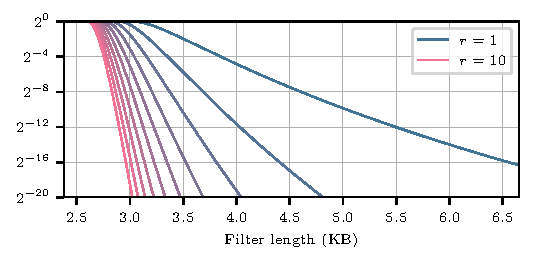
\includegraphics{fig/bf-bound}
  \vspace{-24pt}
  \caption{
    The value of $\zeta_{k,m,n}(q,r)$ (Equation~(\ref{eq:zeta})) for $q=2^{64}$,
    $k=16$, $n=100$, varying values of~$r$ (one line per $r$-value) and filter
    length~$m$ (the x-axis).  Note the log-2 scale on the y-axis.
  }
  \label{fig:bf-bound}
\end{figure}

\begin{proof}[Proof of Theorem~\ref{thm:sbf-errep-immutable}]
  \begin{figure*}
\threeColsOneDivideUnbalanced{0.40}{0.27}{0.27}
{
  \vspace{-7pt}
  \experimentv{$\game_{0}(\advB)$}
      \hfill \diffplus{$\game_1$}\\[2pt]
    $M^* \gets \bot$;
    $\salt^* \getsr \bits^\lambda$\\
    $\advB^{\REPO,\QRYO,\HASHO_1}$;
    return $\big[\sum_x \err[x] \geq r\big]$
  \\[6pt]
  \oraclev{$\REPO(\col)$}\\[2pt]
    $M^* \gets \bigvee_{x \in \col} \bmap_m(\HASHO_2(\salt^* \cat x))$;
    $\setS^* \gets \col$;
    return $\langle M^*, Z^* \rangle$
  \\[6pt]
  \oraclev{$\QRYO(\qry_x)$}\\[2pt]
    $X \gets \bmap_m(\HASHO_3(\salt^* \cat x))$;
    $a \gets X = M^* \AND X$\\
    if $\err[x] < \delta(a,\qry_x(\col^*))$ then
          $\err[x] \gets \delta(a,\qry_x(\col^*))$\\
    return $a$
  \\[6pt]
  \oraclev{$\HASHO_c(\salt \cat x)$}\\[2pt]
    $\vv \getsr [m]^k$\\
    if $M^*=\bot$ and $\salt=\salt^*$ and $c=1$ then \com{Caller is~$\advB$}\\
    \tab $\bad_1 \gets 1$; \diffplus{return $\vv$}\\
    if $T[Z,x] = \bot$ then $\vv \gets T[Z,z]$\\
    $T[Z,x] \gets \vv$; return $\vv$
}
{
  \vspace{-2pt}
  \oraclev{$\HASHO_c(\salt \cat x)$}\\[2pt]
    $\vv \getsr [m]^k$\\
    if $M^*=\bot$ and $\salt=\salt^*$ and $c=1$ then\\
    \tab $\bad_1 \gets 1$; return $\vv$\\
    if $T[Z,x] = \bot$ then $\vv \gets T[Z,z]$\\
    $T[Z,x] \gets \vv$\\[2pt]
    \diffplusbox{
    \com{Caller is~$\advB$ or $\QRYO$}\\
    if $c=1$ or $c=3$ then\\
    \tab if $\salt \ne \salt^*$  then return $\vv$\\
    \tab $\Ans[x] \gets \bmap_m(\vv) = M^* \AND \bmap_m(\vv)$\\
    \tab if $\err[x] < \delta(\Ans[x],\qry_x(\col^*))$ then
    \tab\tab $\err[x] \gets \delta(\Ans[x],\qry_x(\col^*))$
    }
    return $\vv$
}
{
  \vspace{-7pt}
  \oraclev{$\QRYO(\qry_x)$}\
      \hfill \diffminus{$\game_1$} \diffplus{$\game_2$}\\[2pt]
    \diffminusbox{%
      $X \gets \bmap_m(\HASHO_3(\salt^* \cat x))$\\
      $a \gets X = M^* \AND X$\\
      if $\err[x] < \delta(a,\qry_x(\col^*))$ then\\
      \tab $\err[x] \gets \delta(a,\qry_x(\col^*))$
    }\\[2pt]
    \diffplusbox{
      $\HASHO_3(Z^* \cat x)$\\
      $a \gets \Ans[x]$
    }
    return $a$
}
\caption{Games 0, 1, and 2 for proof of Theorem~\ref{thm:sbf-errep-immutable}.}
\label{fig:sbf-errep-immutable/games}
\end{figure*}

We will use the following lemma for keyless structures, which is proved in appendix~\ref{sec:keyless-proof}. We use $\errep1$ and
$\erreps1$ to denote the public-representation and private-representation
experiments where the adversary makes a single $\REPO$ query. In writing the
advantage for these games we omit the $q_R$ parameter since it is fixed at 1.

\begin{lemma}\label{thm:lemma1}
  For every $q_R, q_T, q_U, q_H, r, t \geq 0$ and keyless structure~$\Gamma$ it
  holds that
  \begin{eqnarray*}
    \begin{aligned}
      \Adv{\errep}_{\Gamma,\delta,r}(t, q_R, q_T, q_U, q_H) &\leq \\
      & q_R \cdot \Adv{\errep1}_{\Gamma,\delta,r}(O(f(t)), q_T, q_U, q_H) \,,
    \end{aligned}
  \end{eqnarray*}
  where $f(t) = t + (q_R-1)\ticks(\Rep,t) + q_T\ticks(\Qry,t) + q_U\ticks(\Up,t)$.
\end{lemma}
%
\noindent
The proof is by a fairly straightforward hybrid argument. Because~$\Gamma$ is
keyless, in the reduction we simulate $q_R-1$ of the calls to $\REPO$ experiment
and use our own oracles for the remaining query. The best we can do with this
strategy is to ``guess'' which representation the \errep\ adversary will use in
its attack, which results in the~$q_R$ factor in the bound.
%
We defer the full details to Appendix~\ref{app:iproof/lemma-keyless}.

Let $\advA$ be an \errep\ adversary making~$1$ query to~$\REPO$, $q_T$ queries
to $\QRYO$, $0$ queries to $\UPO$, and $q_H$ queries to the random
oracle~$\HASHO$.
%
We make the following assumptions, all of which are without loss of generality.
%
First, all of~$\advA$'s $\QRYO$ queries proceed its $\REPO$ query.
%
Second, we assume that $x\not\in\setS$ for all queries $\qry_x$ to $\QRYO$,
where~$\setS$ was the input to~$\advA$'s $\REPO$ query. This is without loss
because Bloom filtersadmit false positives, but not false negatives
%
Third, we we assume that $|\setS| \leq n$; this is without loss because
otherwise~$\REPO$ outputs~$\bot$ and~$\advA$ gets no advantage.

Fourth, we assume that all of~$\advA$'s $\HASHO$ queries are of the form $Z\cat
x$, where $|Z| = \lambda$.

We begin with a game-playing argument~\cite{bellare2006triple}, then obtain the
final bound via applicaition of Lemma~\ref{thm:lemma1}.
%
\cpnote{Here's the proof sketch.}
%
The high-level goal is to rewrite the game so that the probability that one
of~$\advA$'s queries runs up the score is precisely the false positive
probability for Bloom filters in the usual analytical
setting~\cite{kirsch2006less}. In other words, our goal is transistion into a
setting in which the Bloom filter output by~$\REPO$ is independent of the
outcome of~$\advA$'s other queries.

We begin with the game~$\game_0(\advB)$ defined in
Figure~\ref{fig:sbf-errep-immutable/games}. It is similar to the \errep\ experiment when
executed with~$\advA$, $\Pi$, $\delta$, and~$r$. Indeed, it is not difficult to
see that for every~$\advA$ there exists an adversary~$\advB$ such that
\begin{equation}
  \Adv{\errep}_{\Pi,\delta,r}(\advA) \leq \Prob{\game_0(\advB) = 1}
\end{equation}
and~$\advB$ has the same query resources as~$\advA$.
%
Adversary~$\advB$ executes~$\advA$, forwarding~$\advA$'s oracle queries
to its own oracles in the natural way.

Observe that in game~$\game_0$ the salt used for the representation of~$\setS^*$
is generated prior to executing~$\advB$. Game~$\game_1$ is identical
to~$\game_0$ until the flag~$\bad_1$ gets set by oracle~$\HASHO$. This occurs
if~$\advB$ asks $\HASHO_1(\salt^* \cat x)$, where~$\salt^*$ is the salt generated
at the beginning of the game, and it has not yet called $\QRYO$ (i.e.,
$M^*=\bot$).
%
By the Fundamental Lemma of Game Playing~\cite{bellare2006triple} it follows
that
%
\begin{eqnarray}
  \Prob{\game_0(\advB)=1} &\leq&
    \Prob{\game_1(\advB)=1} + \Prob{\game_1(\advB) \sets \bad_1}\\
  &\leq&
    \Prob{\game_1(\advB)=1} + q_H/2^\lambda \,.
\end{eqnarray}
%
Note that in $\game_1$, the value of~$M^*$ is independent of~$\advB$'s
$\HASHO_1$ queries. In particular, the probability that some bit of~$M^*$ is set
is independent of the choices of~$\advB$.

In game $\game_2$ the $\HASHO$ and $\QRYO$ oracles have been rewritten so that
the winning-condition is computed by $\HASHO$ instead of $\QRYO$. The former
oracle maintains a set~$\Ans$ such that $\Ans[x] = \Qry^{\HASHO_3}(M^*, x)$ for
each query $\salt^* \cat x$; on input of $\qry_x$, oracle~$\QRYO$ simply runs
$\HASHO_3(\salt^* \cat x)$ and returns $\Ans[x]$.
%
We are effectively giving the adverseary credit for RO queries that result in
false positives for the representation of~$\setS^*$, but which it does not
explicitly ask of the~$\QRYO$. Clearly, for every~$\advB$ it holds that
%
\begin{equation}
  \Prob{\game_1(\advB)=1} \leq \Prob{\game_2(\advB)=1} \,.
\end{equation}

We now consider $\Prob{\game_2(\advB)=1}$.
%
Let $\setX$ be the set $\{ x \in \bits^* : \Ans[x] \ne \bot \}$ and $\setT = \{x
\in\setX: \Ans[x] = 1\}$, where $\Ans$ is at is defined when~$\advB$ halts. We
will call~$\setX$ the set of attempts and~$\setT$ the set of false positives.
%
Note that $\setX\intersection\setS^*=\emptyset$ by construction, and that
$|\setX| \leq q_H + q_T$.
%
Hence, the probability that~$\game_2(\advB)=1$ is equal to the probability
that~$|\setT| \geq r$.

For each $x\in\setX$, let $T(x)$ denote the event that $x\in\setT$
%
In the random oracle model for~$H$, the set of random random variables $T(x)$
for each $x\in X$ are independently and identically distributed.
%
Hence, the probability that~$\advB$ succeeds is binomially distributed:
%
\begin{equation}
  \Prob{ |\setT| \geq r } =
     \sum_{i=r}^{q} \binom{q}{i}p^i(1-p)^{q-i} \,,
\end{equation}
%
where $q \leq q_H + q_T$ and $p = \Pr[T(x)=1]$. Note that the mean $\mu$ of this
distribution is simply $pq$, so we can apply the Chernoff bound with
$\delta = r(pq)^{-1}-1$

If we define
$\alpha = \frac{r}{pq}$, then as long as $\alpha > 1$ we can apply a standard
Chernoff bound to simplify this to
\begin{equation}
  \Prob{ |\setT| \geq r } <
     \left(\frac{e^{\alpha-1}}{\alpha^\alpha}\right)^{pq} \,.
\end{equation}

Substituting this value back in for $\Prob{\game_2(\advB)=1}$ and applying
Lemma~\ref{thm:lemma1} to move from the single-representation case to the
general case, we get our final bound of
\begin{equation}
  \Adv{\errep}_{\Pi,\delta,r}(\advA) < q_R \cdot \left(\frac{q_H}{2^\lambda} + \left(\frac{e^{\alpha-1}}{\alpha^\alpha}\right)^{pq}\right) \,.
\end{equation}

%
\todo{DC (lead)}{Apply Lemma~\ref{thm:lemma1} and finish the bound.}
\end{proof}


Recall that the attack against mutable salted filters exploited the fact that
the adversary learned the salt as soon as the filter was created, and that from
this it could compute the hash function on its own. Even if the filter is
mutable, we can prevent this attack from working as long as we require that the
filter under attack be kept secret from adversaries. In fact, we can attain the
following \erreps\ bound for $\Pi$.

\begin{theorem}[\erreps\ security of salted BFs]\label{thm:sbf-erreps}
  Let $p' = P_{k,m}(n+r)$.
  For all integers $q_R, q_T, q_H, r, t \geq 0$, if
  $r > p'q_T$, then it holds that
  \begin{eqnarray*}
    \begin{aligned}
      \Adv{\erreps}_{\Pi,\delta,r}(t,\,&q_R, q_T, q_U, q_H, q_V) \leq \\
          & q_R \cdot \left[
      \frac{q_H}{2^\lambda} +
      \left(\frac{p'q_T}{r}\right)^re^{r-p'q_T}\right]\,,
    \end{aligned}
\end{eqnarray*}
  where $H$ is modeled as a random oracle.
\end{theorem}

The proof follows a similar structure to that of
Theorem~\ref{thm:sbf-errep-immutable}. The main differences come from arguing
that without a ``lucky'' guess of the salt, the adversary cannot use $\HASHO$ to
find false positives, and from having to show that the adversary's access to
$\UPO$ does not substantially change the security bound that can be derived. The
first of these is straightforward given the private-representation setting, but
the second requires investigating how much of an advantage the $\UPO$ oracle can
give, then moving to games where this advantage is taken into account. We defer
the full proof to Appendix~\ref{sec:proof/sbf-erreps}.

%\begin{proof}[Proof of Theorem~\ref{thm:sbf-erreps}]
%  \begin{figure*}
\cpnote{It should be clear from this figure which boxed statments are included
  in which games. Without the context of the text, the way someone would read
  this is ``gamke 0 includes all unboxed statements; game 1 includes all unboxed
  statments and all boxed statements; and game 2 includes all unboxed and
  gray-boxed statements.'' Please clarify this figure so that it's clear what
  statments are included in what games.}
\twoColsNoDivide{0.47}
{
  \vspace{-7pt}
  \experimentv{$\game_{0}(\advB)$}\\[2pt]
    $M^* \gets \bot$;
    $\salt^* \getsr \bits^\lambda$\\
    $\advB^{\REPO,\QRYO,\UPO,\HASHO_1}$;
    return $\big[\sum_x \err[x] \geq r\big]$
  \\[6pt]
  \oraclev{$\HASHO_c(\salt \cat x)$}\hfill \diffminus{$\game_1$}\\[2pt]
    $\vv \getsr [m]^k$\\
    if $\salt=\salt^*$ and $c = 1$ then \com{Caller is~$\advB$}\\
    \tab $\bad_1 \gets 1$; \diffminus{return $\vv$}\\
    if $T[Z,x] = \bot$ then $\vv \gets T[Z,z]$\\
    $T[Z,x] \gets \vv$; return $\vv$
}
{
  \oraclev{$\QRYO(\qry_x)$}\hfill \diffplus{$\game_2$}\\[2pt]
    $X \gets \bmap_m(\HASHO_3(\salt^* \cat x))$;
    $a \gets X = M^* \AND X$\\
    if $\err[x] < \delta(a,\qry_x(\col^*))$ then
          $\err[x] \gets \delta(a,\qry_x(\col^*))$\\
    \diffplus{$\UPO(\up_x)$}\\
    return $a$
  \\[6pt]
  \oraclev{$\REPO(\col)$}\\[2pt]
    \cpnote{I believe this is incorrect, since $\Rep$ is now thresholding.}
    $M^* \gets \bigvee_{x \in \col} \bmap_m(\HASHO_2(\salt^* \cat x))$;
    $\setS^* \gets \col$;
    return $\top$
  \\[6pt]
  \oraclev{$\UPO(\up_x)$}\\[2pt]
    if $w(M) > \ell$ then return $\top$\\
    if $\QRYO(\qry_x) = 1$ then $\err[x] \gets 0$\\
    $M^* \gets M^* \vee \bmap_m(\HASHO_2(\salt^* \cat x))$;
    $\setS^* \gets \up_x(\setS)$;
    return $\top$
}
\caption{Games 0, 1, and 2 for proof of Theorem~\ref{thm:sbf-erreps}.}
\label{fig:sbf-erreps/games}
\end{figure*}

This proof follows a similar structure to the previous one.
%
\cpnote{Don't refer to thoerems this way; say
Theorem~\ref{thm:sbf-errep-immutable}. That way this reference isn't dangling if
we restructure the paper.}
%
The primary distinction is that in the final game, unless the adversary `gets
lucky' and guesses the salt, they should only be able to produce errors with
$q_T$ queries, as opposed to both $q_T$ and $q_H$ queries.
%
Just as in the proof of Theorem~\ref{thm:sbf-errep-immutable}, we will assume
the adversary just makes a single call to $\REPO$ and use Lemma~\ref{thm:lemma1}
to complete the bound. Let $\advA$ be an \erreps\ adversary making exactly 1
call to $\REPO$, $q_T$ calls to $\QRYO$, $q_U$ calls to $\UPO$, and $q_H$ calls
to $\HASHO$. Because $\advA$ creates only a single representation, it will
necessarily lose if it calls $\REVO$ on that representation. We may therefore
assume without loss of generality that $\advA$ makes no calls to $\REVO$, and
because of this we omit $\REVO$ from each of the games.
%
\cpnote{Good. Somehwere in the body we'll need to justify why we include~$\REVO$
in the experiment, since at this point the reader has no reason to believe that
$\REVO$ captures something useful.}

In addition to the assumptions of the previous theorem \todo{DC}{Fix ref}, we
assume without loss of generality that the adversary never uses $\UPO$ to insert
an element into $\col$ which is already present in the set \todo{DC}{Double
check this assumption isn't made above}, and never uses $\UPO$ to insert an
element $x$ where $\QRYO(\qry_x)$ has already been called and has returned a
positive result. Since these insertions do not change the filter and in the
latter case may actually reduce the error count \cpnote{WHAT?? I don't think
that's true. Remember that the error function is \textbf{fixed} at this point.},
the adversary would gain no advantage from performing these updates.
Furthermore, we assume without loss of generality that an adversary halts as
soon as it determines it has accumulated enough errors to win the experiment.

We begin with a game~$\game_0(\advB)$
(Figure~\ref{fig:sbf-errep-immutable/games}) similar to the previous
proof\todo{DC}{fix ref}, except that it also defines an~$\UPO$ oracle. Again, we
observe that for every~$\advA$ there exists a~$\advB$  such that
\begin{equation}
  \Adv{\errep}_{\Pi,\delta,r}(\advA) \leq \Prob{\game_0(\advB) = 1}
\end{equation}
and~$\advB$ has the same query resources as~$\advA$.

Since we are seeking a stronger bound, we now wish to isolate the possibility
that the adversary \emph{ever} guesses the salt, as opposed to just guessing the
salt before calling $\REPO$. This is no longer a trivial task for the adversary
because the representations are private, and so $\REPO$ does not directly reveal
the salt. We therefore set the~$\bad_1$ flag whenever the adversary manages to
guess the salt, without the requirement that $M^* = \bot$. However, since the
adversary is still limited to a total of $q_H$ $\HASHO$ queries, regardless of
when the queries are made, we can follow nearly the same argument as in the
previous proof to get the bound
%
\begin{eqnarray}
  \Prob{\game_0(\advB)=1} &\leq&
    \Prob{\game_1(\advB)=1} + \Prob{\game_1(\advB) \sets \bad_1}\\
  &\leq&
    \Prob{\game_1(\advB)=1} + q_H/2^\lambda \,.
\end{eqnarray}
%
In~$\game_1$, we may now assume that the adversary never guesses the salt in its $\HASHO_1$ queries. This means that none of the inputs to $\HASHO_1$ is ever equal to any input to $\HASHO_2$ or $\HASHO_3$, both of which always use the salt $\salt^*$. Since each $\HASHO$ is modeled as a random oracle, the outputs of $\HASHO_1$ are therefore independent of the outputs of $\HASHO_2$ and $\HASHO_3$.
%
We still cannot move to the binomial distribution for non-adaptive queries,
however, since $\HASHO_2$ and $\HASHO_3$ queries are not necessarily independent
of each other. By one of our starting assumptions, the same input is never
provided twice to $\HASHO_2$ because the adversary never tries to insert an
element which is already in $\col$. We also argue \cpnote{Do you mean assume?} that (without loss of
generality) the same input is never provided twice to $\HASHO_3$, i.e. that the
same element is never queried twice.

\todo{DC}{Replace $\QRYO(x)$ with $\QRYO(\qry_x)$, here and everywhere else.}
On one hand, if a $\QRYO(x)$ call shows that $x$ is already a false positive for
$\pub$, further $\QRYO(x)$ calls cannot increase the adversary's error score. On
the other hand, if a $\QRYO(x)$ call shows that $x$ is not a false positive, it
is still possible for $x$ to become a false positive later on due to $\UPO$
calls. However, the adversary would obtain at least as large a chance of finding
a false positive by calling $\QRYO(y)$ for some previously unqueried $y
\not\in\col$, since the sequence of updates that could make $x$ a false positive
are just as likely to make $y$ a false positive by the independence of
$\HASHO_c$ calls on different inputs. We can therefore assume that the adversary
does not send repeated queries to $\QRYO$.
%
We have now reduced to a case where all hash queries are independent except for
$\QRYO$ and $\UPO$ calls to the same element. By our starting assumptions, an
adversary never calls $\QRYO$ on an element which has already been inserted, so
we need only consider the case of an element being queried before it is
inserted. In fact, doing this can be beneficial to a pollution attack, since
determining with $\QRYO$ that an element is not already a false positive informs
the adversary that inserting that element must necessarily set at least one new
bit in the filter to 1. Since all other possibilities have been eliminated, we
need only consider two types of update the adversary may make:
%
\begin{enumerate}
  \item Inserting an element which is not already in $\col$ and has previously been tested with $\QRYO$, returning a negative result.
  \item Inserting an element which is not already in $\col$ and has not previously been tested with $\QRYO$.
\end{enumerate}
Since calls to $\HASHO_3$ with different choices of $x$ are independent of each
other, and since $\HASHO_3$ uses random sampling, the effects of type 1 updates
on the representation are identically distributed. Similarly, since calls to
$\HASHO_2$ produce independent random results, the effects of type 2 updates on
the representation are also identically distributed. However, the effects of the
two types of update are \emph{not} identically distributed compared to each
other. In particular, making a type 1 update ensures that at least one new bit
in the filter will be set to 1, since the distribution of
$\bmap_m(\HASHO_2(\salt^* \cat x))$ is conditioned on not producing a false
positive. On the other hand, making a type 2 update provides no guarantee about
how many bits in the filter might be set to 1. Type 1 updates are therefore
always preferable for an adversary attempting to produce false positives.

\cpnote{Got here}
In fact, we can make an even stronger statement: it is always optimal for the
adversary to insert $x$ as soon as $\QRYO(x)$ reveals that $x$ is not a false
positive. Since this is a type 1 update, there is no `better' update which could
benefit the adversary more, so there is no reason for the adversary's next
$\UPO$ call to be anything other than $\UPO(\up_x)$. There is also no reason to
make additional $\QRYO$ calls before calling $\UPO(\up_x)$, since calling
$\UPO(\up_x)$ can only increase the probability that further $\QRYO$ calls
produce an error. We therefore assume without loss of generality that $\advB$
inserts $x$ after $\QRYO(x)$ returns a negative result, provided it still has at
least one $\UPO$ call remaining and this insertion would not increase the size
of the underlying set over the maximum number of $n$ elements.

For~$\game_2(C)$, then, we enforce this behavior, changing $\QRYO(x)$ to automatically insert $x$ into $\col$ after computing the correct response to the query. For any $\advB$ for~$\game_1$ we can construct $C$ for~$\game_2$ that simulates $\advB$ to attain the same advantage, forwarding oracle queries in the natural way except that any call of the form $\UPO(x)$ are ignored if $\QRYO(x)$ has been called previously. Ignoring these $\UPO$ calls does not negatively affect the adversary because in~$\game_2$ the original $\QRYO(x)$ call has already inserted $x$ into the set. Furthermore, the `enhanced' $\QRYO$ available to $C$ does not negatively affect $C$ at any point because inserting additional elements into the filter can only increase the probability that later queries return false positives. Then $C$ wins whenever $\advB$ does, and $\Prob{\game_1(\advB) = 1} \le \Prob{\game_2(C) = 1}$.

However, the parameters of the games played by $C$ and $\advB$ are slightly different. In particular, $\advB$ (and, by extension, $C$) may find up to $r$ false positives before halting. When $\advB$ finds these false positives they are by assumption not ever inserted into $\col$, while in the case of $C$ the $\QRYO$ oracle automatically inserts them into the set as soon as they are found. While inserting a false positive does not affect the filter itself in any way, it does increment the number of elements in the underlying set. Therefore if adversaries $\advB$ in~$\game_1$ are limited to representing a set of size $n$, we restrict adversaries $C$ in~$\game_2$ to representing sets of up to size $n+r$.

In~$\game_2$, $\UPO$ queries are actually superfluous. Since every element queried is automatically inserted into the set and the adversary never inserts an element more than once, $\UPO$ calls are now all of type 2. Since these insertions can only increase the chance of each following $\QRYO$ call being a false positive, it is optimal for the adversary to make all $\UPO$ calls at the beginning of the experiment, and then to make all $\QRYO$ calls. But this means we can assume without loss of generality that the adversary makes no $\UPO$ calls at all, since any elements added through $\UPO$ before any $\QRYO$ calls are made could just as easily have been included in the original call to $\REPO$ without affecting the adversary's advantage.

We now therefore only consider the case of a $\REPO$ call followed by the~$\game_2$ version of $\QRYO$ calls. Let $\setX$ be the set of all queries $\qry_x$ which are sent to $\QRYO$ over the course of the experiment. We necessarily have $|\setX| \le q_T$, and each $\qry_x \in \setX$ has some probability of causing an error. Since $\col^*$ never grows to contain more than $n+r$ elements, the false positive probability for each such $\qry_x$ is bounded above by $p_*$, the false-positive probability of a Bloom filter containing $n+r$ elements. So we have, analagously to the previous theorem,
\begin{equation}
   \Prob{\game_2(\advB)=1} \le
     \sum_{i=r}^{q_T} \binom{q_T}{i}p_*^i(1-p_*)^{q_T-i} \,,
\end{equation}
where $q_T$ replaces $q$ and the larger $p_*$ replaces $p$. Applying the same Chernoff bound reduces this to
\begin{equation}
   \Prob{\game_2(\advB)=1} \le
     e^{r-p_*q_T}\left(\frac{p_*q_T}{r}\right)^r.
\end{equation}

Again we apply Lemma~\ref{thm:lemma1} to get a final bound of
\begin{equation}
  \Adv{\erreps}_{\Pi,\delta,r}(\advA) \leq
    q_R \cdot \left[
      \frac{q_H}{2^\lambda} +
      \left(\frac{p_*q_T}{r}\right)^re^{r-p_*q_T}
    \right] \,.
\end{equation}

%\end{proof}

\subsection{Keyed BFs}

Salted BFs are \erreps\ secure in general, and are \errep\ secure in the
immutable setting, but are not \errep\ secure when the adversary has access to
an $\UPO$ oracle. Our argument for the \erreps\ security of
salted Bloom filters is made possible by virtue of the structure under attack
not being revealed to the adversary. While this is realistic in many
applications, it may be desirable for the Bloom filter to be public \emph{and}
updatable.
%
Here we show that building a Bloom filter from a PRF suffices for security in
this setting.
%
Let $F:\keys\by\bits^*\to[m]^k$ be a function, fix
integers~$n,\lambda\geq0$, and let $\Pi = \KBF[F,n,\lambda]$.

\begin{theorem}[\errep\ security of keyed BFs]
\label{thm:bf-key-bound}
\label{thm:kbf-errep}
  Let $p' = P_{k,m}(n+r)$.  For integers $q_R, q_T, q_H, r, t \geq 0$ such that
  $r > p'q_T$, it holds that
  \begin{equation*}
    \begin{aligned}
      \Adv{\errep}_{\Pi,\delta,r}(t,\,&q_R,q_T,q_U,q_H) \leq \\
        \Adv{\prf}_F(O(t),nq_R+q_T+q_U) & +
      \frac{q_R^2}{2^\lambda} +
      \left(\frac{p'q_Rq_T}{r}\right)^re^{r-p'q_Rq_T} \,.
    \end{aligned}
  \end{equation*}
\end{theorem}

As usual, our strategy will be to move to the non-adaptive setting via a
sequence of game transitions.  The details of we get there differ from the
keyless Bloom filters.  In particular, since we are using a PRF, the initial
parts of the proof deal with the adversary potentially being able to break the
PRF and with the possibility of the salts repeating rather than with the
adversary being able to guess the salt.
%
We defer the details to Appendix~\ref{sec:proof/kbf-errep}.

%\begin{proof}
%  \begin{figure*}
\todo{DC}{nit: Here and throughout the rest of paper, change $ct$ to
$\mathit{ct}$. The former looks like $c\cdot t$.}
\twoCols{0.47}
{
  \vspace{-7pt}
  \experimentv{$\game_{0}(\advA)$}\\[2pt]
    $\key \getsr \keys$;
    $ct \gets 0$\\
    $i \getsr \advA^{\REPO,\QRYO,\UPO}$;
    return $\big[\sum_x \err_i[x] \geq r\big]$
  \\[6pt]
  \oraclev{$\PRFO(\salt \cat x)$}\hfill\diffminus{$\game_0$}\diffplus{$\game_1$}\\[2pt]
    \diffminus{$\vv \gets F_K(\salt \cat x)$}\\
    \diffplusbox{$\vv \getsr [m]^k$\\
    if $T[Z,x] = \bot$ then $\vv \gets T[Z,z]$\\
    $T[Z,x] \gets \vv$; return $\vv$}
  \\[6pt]
  \oraclev{$\QRYO(i, \qry_x)$}\\[2pt]
    $X \gets \bmap_m(\PRFO(\salt_i \cat x))$;
    $a \gets X = M_i \AND X$\\
    if $\err_i[x] < \delta(a,\qry_x(\col_i))$ then
          $\err_i[x] \gets \delta(a,\qry_x(\col_i))$\\
    return $a$
  \\[6pt]
  \oraclev{$\REPO(\col)$}\\[2pt]
    $ct \gets ct+1$;
    $\setS_{ct} \gets \col$;
    $\salt_{ct} \getsr \bits^\lambda$;
    $c_{ct} \gets |\col|$\\
    $M_{ct} \gets \bigvee_{x \in \col} \bmap_m(\PRFO(\salt_{ct} \cat x))$;
    return $\langle M_{ct}, \salt_{ct}, c_{ct} \rangle$
  \\[6pt]
  \oraclev{$\UPO(i, \up_x)$}\\[2pt]
    if $w(M) > \ell$ then return $\top$\\
    if $\QRYO(\qry_x) = 1$ then $\err_i[x] \gets 0$\\
    $M_i \gets M_i \vee \bmap_m(\PRFO(\salt_i \cat x))$;
    $\setS_i \gets \up_x(\setS_i)$;
    return $\langle M_i, \salt_i, c_i+1\rangle$
}
{
  \vspace{-7pt}
  \experimentv{$\game_2(\advA)$}\hfill\diffplus{$\game_3$}\\[2pt]
    $\key \getsr \keys$;
    $ct \gets 0$;
    $\setZ \gets \emptyset$\\
    $i \getsr \advA^{\REPO,\QRYO,\UPO}$;
    return $\big[\sum_x \err_i[x] \geq r\big]$
  \\[6pt]
  \oraclev{$\REPO(\col)$}\\[2pt]
    $ct \gets ct+1$;
    $\setS_{ct} \gets \col$;
    $\salt_{ct} \getsr \bits^\lambda \setminus \setZ$;
    $c_{ct} \gets |\col|$\\
    $\setZ \gets \setZ \cup \{\salt_{ct}\}$\\
    $M_{ct} \gets \bigvee_{x \in \col} \bmap_m(\PRFO(\salt_{ct} \cat x))$;
    return $\langle M_{ct}, \salt_{ct}, c_{ct} \rangle$
  \\[6pt]
  \oraclev{$\QRYO(i, \qry_x)$}\\[2pt]
    $X \gets \bmap_m(\PRFO(\salt_i \cat x))$;
    $a \gets X = M_i \AND X$\\
    if $\err_i[x] < \delta(a,\qry_x(\col_i))$ then
          $\err_i[x] \gets \delta(a,\qry_x(\col_i))$\\
    \diffplus{$\UPO(i, \up_x)$;}
    return $a$
  \\[4pt]
  \hrule
  \vspace{2pt}
  \oraclev{$\QRYO(i, \qry_x)$}\hfill\diffminus{$\game_3$}\diffplus{$\game_4$}\\[2pt]
    \diffminusbox{
    $X \gets \bmap_m(\PRFO(\salt_i \cat x))$;
    $a \gets X = M_i \AND X$\\
    if $\err_i[x] < \delta(a,\qry_x(\col_i))$ then
          $\err_i[x] \gets \delta(a,\qry_x(\col_i))$\\
    $\UPO(i, \up_x)$;
    return $a$
    }
    \diffplusbox{
    for $j \in [ct]$ do\\
    $\tab X \gets \bmap_m(\PRFO(\salt_j \cat x))$;
    $a_j \gets X = M_j \AND X$\\
    $\tab$if $\err_j[x] < \delta(a_j,\qry_x(\col_j))$ then
          $\err_j[x] \gets \delta(a_j,\qry_x(\col_j))$\\
    $\tab\UPO(j, \up_x)$\\
    return $a_i$}
}
\caption{Games 0--4 for proof of Theorem~\ref{thm:bf-key-bound}.}
\label{fig:kbf-errep/games}
\end{figure*}

We start with a game~$\game_0$ which is essentially the same as the standard
\errep\ experiment on a Bloom filter, given the assumption (without loss of
generality) that the adversary never attempts to construct a representation for
a set with more than $n$ elements. As with the other proofs, it is easy to see
that for any such \errep\ adversary we can make an adversary $\advA$
for~$\game_0$ with the same resources that achieves the same advantage.

Unlike in the previous two proofs, we cannot use Lemma~\ref{thm:lemma1} because
an adversary cannot simulate the oracles without knowing the private key. We use
an alternate approach to gradually reduce to the standard binomial bound
deriving from the non-adaptive false positive probabilities. The first thing we
want to do is to bound the probability that the adversary can break the PRF.

The number of times the PRF is evaluated on distinct inputs is bounded by the
number of queries available to the adversary. In particular, $\QRYO$ and $\UPO$
each call the PRF once, while $\REPO$ may call the PRF up to $n$ times. If the
adversary runs in $t$ time steps, then, the probability it can distinguish the
PRF from a random function is bounded by $\Adv{\prf}_F(t,nq_R+q_T+q_U)$.
%
In~$\game_1$, we have a game which is identical to~$\game_0$ except that it uses
random sampling in place of the PRF. If $\advA$ cannot distinguish the PRF from
a random function then these games are indistinguishable from the adversary's
perspective, so $\Prob{\game_0(\advA) = 1} \le \Adv{\prf}_F(t,nq_R+q_T+q_U) +
\Prob{\game_1(\advA) = 1}$.
%
\cpnote{In fat, this isn't immediate. You show this by a reduction. You want to
show that for every $\advA$ there exists an adversary~$D$ such that
$\Prob{\game_0(\advA)=1} - \Prob{\game_1(\advA)=1} \leq \Adv{\prf}_F(D)$. You
don't need to be super formal about it, but you do need to say how~$D$
executes~$\advA$ and what outputs.}

Our goal is to argue, in a similar manner as to the previous theorems, that all of the oracle calls are independent. In order to guarantee this we must deal with the possibility of a salt collision between different representations. In~$\game_2(\advA)$ we require that all salts be distinct between representations. By the birthday bound, collisions between randomly-generated salts occur with frequency at most $q_R^2/2^\lambda$, so $\Prob{\game_1(\advA) = 1} \le q_R^2/2^\lambda + \Prob{\game_2(\advA) = 1}$.

With guaranteed-unique salts, the result of each $\REPO$, $\UPO$, and $\QRYO$
call for a given representation is independent of the calls for all other
representations. By an almost identical argument to the one in the proof of
Theorem~\ref{thm:sbf-erreps}, we can reduce from any $\advA$ to an adversary
$\advB$ which follows any $\QRYO$ call that finds a true negative with an
$\UPO$ call to insert that element, and therefore move to~$\game_3(\advB)$,
which as in the Theorem~\ref{thm:sbf-erreps} proof performs an update after each
query is made, with the guarantee that $\Prob{\game_1(\advA) = 1} \le \Prob{\game_2(\advB) = 1}$

Finally, we must deal with the possibility that the adversary chooses which
representations to target with $\UPO$ and $\QRYO$ calls based on the result of
$\REPO$, since some representations may be more full than others. In
game~$\game_4$, we allow the adversary credit if a call to
$\QRYO$ produces an error in any of the representations that have been
constructed. Furthermore, the updates made by $\QRYO$ apply to all
representations that are not already full. Since all $\UPO$ calls are
identically and independently distributed, and having more elements in a filter
cannot decrease the false positive rate, the fact that some representations may
become full more quickly than they otherwise would have can only help the
adversary. Similarly, having $\QRYO$ count errors across all representations
never harms the adversary, and so the adversary's advantage may only increase
when moving to~$\game_4$,
i.e. $\Prob{\game_3(\advB) = 1} \le \Prob{\game_4(\advB) = 1}$.

We are now in a situation where we can apply the standard, non-adaptive error
bound. Let $\setX$ be the set of all queries $\qry_x$ made by the adversary over
the course of the game. As in the previous proof, we have $|\setX| \le q_T$.
However, $\qry_x$ may now cause a false positive in any of the representations.
The probability of causing a false positive in a specific representation is
still given by the non-adaptive false positive probability $p'$ for a Bloom
filter containing $n+r$ elements. Since the representations are independent of
each other, the probability of a false positive occurring in any of up to $q_R$
representations is at most $p'q_R$. We can therefore bound the adversary's
success probability using a binomial distribution, similar to before:
\begin{equation}
   \Prob{\game_4(\advB)=1} \le
     \sum_{i=r}^{q_T} \binom{q_T}{i}(p'q_R)^i(1-p'q_R)^{q_T-i} \,.
\end{equation}

Applying the usual Chernoff bound, we find
\begin{equation}
   \Prob{\game_4(\advB)=1} \le
     e^{r-p'q_Rq_T}\left(\frac{p'q_Rq_T}{r}\right)^r.
\end{equation}

So, substituting this bound back into the earlier advantage inequalities, we find the final bound of
\begin{equation*}
  \begin{aligned}
    \Adv{\errep}_{\Pi,\delta,r}(t, q_R,q_T,q_U,q_H) &\leq \\
      \Adv{\prf}_F(t,nq_R+q_T+q_U) & +
    \frac{q_R^2}{2^\lambda} +
    \left(\frac{p'q_Rq_T}{r}\right)^re^{r-p'q_Rq_T}
  \end{aligned}
\end{equation*}
%\end{proof}

The fact that both a key and a salt are used in the $\KBF$ construction is
critical. In particular, without the per-representation randomness given by the
salt, we would not be able to argue that $\UPO$ and $\QRYO$ calls are
independent across representations. On the contrary, seeing the representation
of a singleton set $\{x\}$ would immediately allow the adversary to test whether
$x$ was a member in every other representation that had been constructed, simply
by testing whether every bit set to $1$ in the representation of $\{x\}$ was also
set to 1 in other representations. Even in the \erreps\ game, using the $\REVO$
oracle on some representations leaks information about other representations,
and again we cannot use the argument that provides the above bound.

We note that Gerbet \etal~\cite{gerbet2015power} suggest using keyed
hash functions as one possibility for constructing secure filters, which is
equivalent in our terminology to using a keyed but unsalted filter.
%
The distinction is that Gerbet \etal assume that representations are kept
private indefinitely, an assumption similar to that underlying our \erreps\
game, but with the stronger restriction that the adversary has no equivalent of
a $\REVO$ oracle. This makes their notion of security much weaker than ours with
respect to keyed structures.

\subsection{$\ell$-thresholded BFs}\label{sec:bf-thresh}

\begin{figure}
  \twoColsNoDivide{0.22}
  {
    \underline{$\Rep^R_K(\col)$}\\[2pt]
      $\salt \getsr \bits^\lambda$;
      $\pub \gets \langle 0^m, \salt\rangle$\\
      for $x \in \col$ do\\
        $\tab \pub \gets \Up^R_K(\pub,\qry_x)$\\
        $\tab$if $\pub = \bot$ then return $\bot$\\
      return $\pub$
  }
  {
    \underline{$\Qry^R_K(\langle M, \salt \rangle,\qry_x)$}\\[2pt]
      $X \gets \bmap_m(R_K(\salt \cat x))$\\
      return $M \AND X = X$
    \\[6pt]
    \underline{$\Up^R_K(\langle M, \salt \rangle,\qry_x)$}\\[2pt]
      if $\hw(M) > \ell$ then return $\bot$\\
      return $\langle M \vee \bmap_m(R_K(\salt \cat x)), \salt \rangle$
  }
  \caption{The class of $\ell$-thresholded Bloom filters is given by
  $\bloom_\mathrm{ft}[R,\ell,\lambda] = (\Rep^R,\Qry^R,\Up^R)$. This is a slight
  variant of $n$-capping wherein we use the Hamming weight of the filter ($\hw$,
  as defined in Section~\ref{sec:prelims}) to decide if the filter is full.}
  \label{fig:bft-def}
\end{figure}

So far we have proven bounds for only $n$-capped BFs. It is important to understand
the security of this class of structures because it is representative of
how BFs are used in practice.
%
In this section we demonstrate show that we improve security bounds by defining
``fullness'' in terms of the weight of the filter, rather than the number of
elements it represents.
%
The general form of this alternate construction is formally defined in
Figure~\ref{fig:bft-def}. We can define the more specific constructions
$\BF_\mathrm{ft}[H,\ell]$, $\SBF_\mathrm{ft}[H,\ell,\lambda]$, and
$\KBF_\mathrm{ft}[H,\ell,\lambda]$ in an exactly the same way as the $n$-capped
variants. Here we only consider case of
$\Pi = \SBF_\mathrm{ft}[H,\ell,\lambda]$ and compare it to the $\SBF$
construction in Section~\ref{sec:sbf}.
%
The non-adaptive false positive probability is similar is similar to capped
filters, since the number of~$1$ bits in the filter can be closely predicted
from the number of elements in a randomly-selected underlying set. Because of
this, and because we are able to demonstrate better security bounds for an
$\ell$-thresholded filter than for a capped filter, we suggest this as a way
of providing strong security guarantees for even smaller filter sizes.

\begin{theorem}[\erreps\ security of thresholded BFs]\label{thm:bf-thr-bound}
Let $p_\ell = ((\ell+k)/m)^k$. For integers $q_R, q_T, q_H, r, t \geq 0$ such
that $r > p_\ell q_T$, it holds that
  \begin{equation*}
    \begin{aligned}
      \Adv{\erreps}_{\Pi,\delta,r}(t,\,&,q_R,q_T,q_U,q_H,q_V) \leq \\
        & \frac{q_R(q_H+q_R)}{2^\lambda} + e^{r-p_\ell q_T}\left(\frac{p_\ell q_T}{r}\right)^r
        \,,
    \end{aligned}
  \end{equation*}
  where~$H$ is modeled as a random oracle.
\end{theorem}

From a technical point of view, the main difference between thresholded and
capped filters is that attacks cannot set more than $\ell+k$ bits of the filter
to 1, regardless of how the attack is conducted. The thrust of the proof is to
assume the adversary will always be able to produce such a maximally full
filter, and then use a standard binomial-distribution-based bound to place a
limit on the adversarial advantage even in this worst-case scenario.

\todo{CP}{If time, plot the bound just like before and compare it to
Theorem~\ref{thm:sbf-erreps}.}

\begin{proof}
  \begin{figure*}
\twoCols{0.47}
{
  \vspace{-7pt}
  \experimentv{$\game_{0}(\advA)$}\hfill\diffminus{$\game_0(\advA)$}\diffplus{$\game_1(\advB)$}\\[2pt]
    $ct \gets 0$;
    $\setZ \gets \emptyset$;
    $\setP \gets \emptyset$\\
    \diffminus{$i \gets \advA^{\REPO,\QRYO,\UPO,\HASHO_1,\REVO}$}\\
    \diffplus{$i \gets \advB^{\REPO,\QRYO,\UPO,\HASHO_1}$}\\
    return $\big[\sum_x \err_i[x] \geq r\big] \wedge i \not\in \setP$
  \\[6pt]
  \oraclev{$\HASHO_c(\salt \cat x)$}\\[2pt]
    $\vv \getsr [m]^k$\\
    if $\salt \in \setZ$ and $c = 1$ then \com{Caller is adversary}\\
    \tab $\bad_1 \gets 1$\\
    if $T[Z,x] = \bot$ then $\vv \gets T[Z,z]$\\
    $T[Z,x] \gets \vv$; return $\vv$
  \\[6pt]
  \oraclev{$\QRYO(i, \qry_x)$}\\[2pt]
    $X \gets \bmap_m(\HASHO_3(\salt_i \cat x))$;
    $a \gets X = M_i \AND X$\\
    if $\err_i[x] < \delta(a,\qry_x(\col_i))$ then
          $\err_i[x] \gets \delta(a,\qry_x(\col_i))$\\
    return $a$
  \\[6pt]
  \oraclev{$\REPO(\col)$}\hfill \diffplus{$\game_1$}\\[2pt]
    $ct \gets ct+1$;
    $M_{ct} \gets 0^m$;
    $\salt_{ct} \gets \bits^\lambda$\diffplus{$\setminus \setZ$}\\
    \diffplus{$\setZ \gets \setZ \cup \{\salt_{ct}\}$;}
    $\setS_{ct} \gets \col$\\
    for $x \in \col$ do\\
    $\tab\UPO(ct, \up_x)$\\
    return $\top$
  \\[6pt]
  \oraclev{$\UPO(i, \up_x)$}\\[2pt]
    if $w(M) > \ell$ then return $\top$\\
    if $\QRYO(\qry_x) = 1$ then $\err_i[x] \gets 0$\\
    $M_i \gets M_i \vee \bmap_m(\HASHO_2(\salt^* \cat x))$;
    $\setS_i \gets \up_x(\setS_i)$
    return $\top$
  \\[6pt]
  \oraclev{$\REVO(i)$}\\[2pt]
    $\setP \gets \setP \cup \{i\}$\\
    return $\langle M_i, \salt_i\rangle$
}
{
  \vspace{-7pt}
  \oraclev{$\HASHO_c(\salt \cat x)$}\hfill\diffplus{$\game_2$}\\[2pt]
    $\vv \getsr [m]^k$\\
    if $\salt \in \setZ$ and $c = 1$ then \com{Caller is adversary}\\
    \tab $\bad_1 \gets 1$; \diffplus{return $\vv$}\\
    if $T[Z,x] = \bot$ then $\vv \gets T[Z,z]$\\
    $T[Z,x] \gets \vv$; return $\vv$

  \vspace{6pt}\hrule\vspace{3pt}

  \oraclev{$\REPO(\col)$}\hfill\diffplus{$\game_3$}\\[2pt]
    $ct \gets ct+1$;
    $M_{ct} \gets 0^m$;
    $\salt_{ct} \gets \bits^\lambda\setminus \setZ$\\
    $\setZ \gets \setZ \cup \{\salt_{ct}\}$;
    $\setS_{ct} \gets \col$\\
    for $x \in \col$ do\\
    $\tab\UPO(ct, \up_x)$\\
    \diffplusbox{while $w(M_{ct}) < \ell+k$ do\\
    $\tab i \getsr [m]$;
    $M_{ct}[i] \gets 1$}
    return $\top$

  \vspace{6pt}\hrule\vspace{3pt}

  \experimentv{$\game_4(D)$}\\[2pt]
    $M \gets 0^m$\\
    while $w(M_{ct}) < \ell+k$ do\\
    $\tab i \getsr [m]$;
    $M_{ct}[i] \gets 1$\\
    $D^{\QRYO}$;
      \cpnote{Where's $D$'s $\HASHO_1$ oracle?}\\
    return $\big[\sum_x \err[x] \geq r\big]$
  \\[6pt]
  \oraclev{$\QRYO(\qry_x)$}\\[2pt]
    $X \gets \bmap_m(\HASHO_3(\salt_i \cat x))$\\
    $a \gets X = M \AND X$\\
    $\err[x] \gets a$\\
    return $a$
}
\caption{Games 0, 1, and 2 for proof of Theorem~\ref{thm:sbf-erreps}.}
\label{fig:sbf-erreps/games}
\end{figure*}

As in previous proofs, we assume without loss of generality that there are no
insertions of or queries for elements of $\col$, and we start with a
game~$\game_0$ that is identical to the \erreps\ game for $\KBF_\mathrm{ft}$.
\cpnote{Where is~$\game_0$? Refer to the figure.}

To avoid the unfortunate $q_R$ factor in the bound, we do not make use of
Lemma~\ref{thm:lemma1} in this proof. Because of that, we must find some other
way to ensure that $\REVO$ is not useful to the adversary. In particular, if
there are unique salts across representations, the $\REPO$, $\QRYO$, and $\UPO$
calls for one representation will be independent of those for other
representations, since the unique salt is passed as part of the input. Therefore
in~$\game_1$ we specify that all salts created will be unique, but deny access
to $\REVO$. By the birthday bound, the probability of salts repeating
in~$\game_0$ is no more than $q_R^2/2^\lambda$. If the representations are
independent, calling $\REVO$ would provide no information about other
representations, and would in fact only weaken the adversary by causing some
possible outputs $i \in [q_R]$ to be automatic losses. So we have
$\Prob{\game_0(\advA) = 1} \le q_R^2/2^\lambda + \Prob{\game_1(\advB) = 1}$,
where $\advB$ is an adversary that performs identically to $\advA$ but is
syntactically distinct because it lacks a $\REVO$ oracle.

Next, we want to ensure that the adversary's $\HASHO_1$ queries are independent
of the $\HASHO_2$ and $\HASHO_3$ queries used for $\REPO$, $\QRYO$, and $\UPO$.
Since the $\HASHO_c$ oracles use random sampling to fill a shared table, this
occurs if and only if the adversary calls
$\HASHO_1(\langle\salt_i,x\rangle)$\todo{DC}{Fix syntax}
for some salt $\salt_i$ used by one of the representations created by $\REPO$.
By an argument very similar to that in the previous proofs, the adversary has at
most $q_H/2^\lambda$ probability of calling $\HASHO_1$ with the salt used by
some specific representation. However, since there are now $q_R$
representations, each with a distinct salt, there is at most a
$q_Rq_H/2^\lambda$ probability of the adversary correctly guessing a salt.
In~$\game_1(\advB)$, we set the $\bad_1$ flag if the adversary succeeds in
guessing the salt in this manner, but the flag does not affect the game. The
case of~$\game_2(\advB)$ is identical until the $\bad_1$ flag is set, which
occurs only when a salt is guessed, so we have $\Prob{\game_1(\advB) = 1} \le
q_Rq_H/2^\lambda + \Prob{\game_2(\advB) = 1}$.

We may now assume~\cpnote{Actually, this is by \textbf{construction}! In the
revised game, the adversary is never handed the correct salt, and it's never
handed any RO output whose input is preprended by the salt. it's not the
aadversary never ``guesses'' it, it's that it doesn't matter if it does! This
the real power game-based proofs. Please revise this, here and elsehwere.} that
the adversary never guesses the salt of any of the
representations, and so the outputs of $\HASHO_1$ are independent of the results
of all calls to $\REPO$, $\QRYO$, and $\UPO$. The next oracle we want to target
is $\UPO$. Now that we have a filter threshold, we want to argue that the
adversary cannot use $\UPO$ to mount an effective pollution attack.
%
\cpnote{You're implicitly assuming that pollution attacks are the best we can
do. Why is this true? It doesn't seem to me like it's true. Maybe it is at this
point in the proof, because we've already dealt with the salt guessing? If
that's the case, we can't call it a ``pollution attack'', since this the
experiment has changed.}
%
In~$\game_3(C)$, the $\REPO$ oracle creates the filter as normal and then
randomly sets bits until filter is full (i.e., its Hamming weight is at least
$\ell$), which is $\ell+k$ (since
updates are not allowed when more than $\ell$ bits are set, and a single update
may set at most $k$ bits to 1). For any $\advB$ in~$\game_2$, we can construct
$C$ for~$\game_3$ that obtains at least as large an advantage by having $C$
simulate $\advB$, forwarding all oracle queries in the natural way except that
$\UPO$ queries are ignored, with $C$ simply returning $\top$ to $\advB$ without
performing any additional computations or oracle calls. (Recall that, in the
\erreps setting, the adversry expects $\top$ to be the output of~$\UPO$.) Since $\advB$ does not
query elements which are already in $\col$, the outputs of $\HASHO_3$ calls are
independent of any prior $\HASHO_2$ calls.
%
The probability of such an output producing a false positive is strictly a
function of the number of bits in the filter which have been set to 1.
%
Since at least as many bits have been set to 1 in~$\game_3$ as in~$\game_2$,
every $\QRYO$ call is at least as likely to produce a false positive. Therefore
$\Prob{\game_2(\advB) = 1} \le \Prob{\game_3(C) = 1}$.

In~$\game_3$ we can assume without loss of generality that the adversary makes
no $\UPO$ calls, since the filter is already full and no additional updates will
be accepted. \cpnote{Why assume this? The adversary can make as many $\UPO$
queries it wants and it won't make a difference. So why stop it? The reason not
to is that, as a general good, it's good to keep your assumptions minimal.} Since each
representation is created using independent $\HASHO_2$ outputs and then filled
in a uniform random manner until $\ell+k$ bits are set to 1, and is never
modified afterwards, the representations
themselves are random bitmaps which are uniformly distributed over the set of
$m$-length bitmaps with $\ell+k$ bits set to 1. This allows us to move
to~$\game_4(D)$, where the adversary is given a single arbitrary bitmap $\pub$
of length $m$ with $\ell+k$ bits set to 1 and makes $\QRYO$ calls exclusively
for $\pub$, winning if it produces $r$ errors for that `representation'. Given
an adversary $C$ for~$\game_3$, we construct a $D$ for~$\game_4$ that simulates
$C$. When $C$ makes a $\REPO$ call, $D$ immediately returns $\top$ to $C$, and
when $C$ makes a $\QRYO(i,\qry_x)$ call, $D$ selects a random
previously-unqueried element $y$ and calls $\QRYO(y)$, returning the result to
$C$. \cpnote{What about~$C$'s $\HASHO_1$ queries?} Since representations are uniformly distributed and $\HASHO_3$ calls are
independent of the $\HASHO_2$ calls used to construct the representation, each
$\QRYO$ call made by $D$ has the same chance of producing a hit as the $\QRYO$
call made by $C$ has of producing a false positive.
%
\cpnote{What about queries $(i,\qry_x)$ and $(j,\qry_x)$? $D$'s response will be
the same for both, but $C$ is expecting independent outputs.}
%
The win conditions differ
only in that $D$ wins by accumulating $r$ positive results, whereas $C$ must
accumulate $r$ false positives within a single representation, and so $D$ wins
if $\advB$\todo{DC}{You mean $C$?} does. Therefore $\Prob{\game_3(C) = 1} \le \Prob{\game_4(D) = 1}$.

However, since $\QRYO$ calls with distinct inputs have independent outputs, each $\QRYO$ call made by $D$ has the same probability of producing a false positive. In particular, the probability of any one of the $k$ outputs of $\HASHO_3$ colliding with a 1 bit is $(\ell+k)/m$, and the probability of all $k$ outputs doing so is then $((\ell+k)/m)^k$. If we let $\setX$ be the set of all inputs made to $\QRYO$, we again have a binomial distribution where $q_T$ queries are made. Letting $p_\ell = ((\ell+k)/m)^k$, we have
\begin{equation}
   \Prob{\game_4(D)=1} \le
     \sum_{i=r}^{q_T} \binom{q_T}{i}p_\ell^i(1-p_\ell)^{q_T-i} \,,
\end{equation}
and we can once more apply a Chernoff bound, as long as $p_\ell q_T < r$, to simplify this to
\begin{equation}
   \Prob{\game_4(D)=1} \le
     e^{r-p_\ell q_T}\left(\frac{p_\ell q_T}{r}\right)^r.
\end{equation}

Substituting this into our earlier inequalities yields the final bound of
\begin{equation}
   \Adv{\erreps}_{\Pi,\delta,r}(\advA) \leq
     \frac{q_R(q_H+q_R)}{2^\lambda} + e^{r-p_\ell q_T}\left(\frac{p_\ell q_T}{r}\right)^r.
\end{equation}

\end{proof}


\subsection{Discussion}

These results show that the standard Bloom filter construction is not secure
against an adaptive adversary. The best mitigation strategy against potential
attacks depends on the setting. If Bloom filters are designed to be immutable,
using a per-representation salt and a sufficiently large filter is sufficient.
Similarly, if the filters are not revealed to potential adversaries (i.e.
parties that get to choose inputs), salting provides a security guarantee which
can be further improved by using $\ell$-thresholding. Importantly, if filters
cannot be kept private, a secret key must be used alongside the salt to prevent
potential attacks.

These requirements are more stringent than the mitigations suggested by Gerbet
\etal~\cite{gerbet2015power} due to our stronger attack model (where multiple
filters can be constructed, and sometimes revealed, to the adversary) and our
goal of establishing a general security bound for any adversary rather than
mitigating specific attacks. If $q_R$ is small, our \erreps\ guarantee for
$\SBF$ and \errep\ guarantee for $\KBF$ show that filters need not be made much
larger than Gerbet \etal's in order to provide comparable security against more
general adversaries. If $q_R$ is large, however, the $q_R$ term in the error
bounds means that the filters must be made large to provide good error
guarantees. In this scenario, however, the $\ell$-thresholding class of filter
provides a way to get strong error guarantees without significantly increasing
the filter size.

\cpnote{How does the $\ell$-threshold bound compare to that of $n$-capping?}
\dcnote{This should probably be a graph, but I can't get pylab working for some
reason...}